% Options for packages loaded elsewhere
\PassOptionsToPackage{unicode}{hyperref}
\PassOptionsToPackage{hyphens}{url}
%
\documentclass[
]{article}
\usepackage{amsmath,amssymb}
\usepackage{iftex}
\ifPDFTeX
  \usepackage[T1]{fontenc}
  \usepackage[utf8]{inputenc}
  \usepackage{textcomp} % provide euro and other symbols
\else % if luatex or xetex
  \usepackage{unicode-math} % this also loads fontspec
  \defaultfontfeatures{Scale=MatchLowercase}
  \defaultfontfeatures[\rmfamily]{Ligatures=TeX,Scale=1}
\fi
\usepackage{lmodern}
\ifPDFTeX\else
  % xetex/luatex font selection
\fi
% Use upquote if available, for straight quotes in verbatim environments
\IfFileExists{upquote.sty}{\usepackage{upquote}}{}
\IfFileExists{microtype.sty}{% use microtype if available
  \usepackage[]{microtype}
  \UseMicrotypeSet[protrusion]{basicmath} % disable protrusion for tt fonts
}{}
\makeatletter
\@ifundefined{KOMAClassName}{% if non-KOMA class
  \IfFileExists{parskip.sty}{%
    \usepackage{parskip}
  }{% else
    \setlength{\parindent}{0pt}
    \setlength{\parskip}{6pt plus 2pt minus 1pt}}
}{% if KOMA class
  \KOMAoptions{parskip=half}}
\makeatother
\usepackage{xcolor}
\usepackage[margin=1in]{geometry}
\usepackage{color}
\usepackage{fancyvrb}
\newcommand{\VerbBar}{|}
\newcommand{\VERB}{\Verb[commandchars=\\\{\}]}
\DefineVerbatimEnvironment{Highlighting}{Verbatim}{commandchars=\\\{\}}
% Add ',fontsize=\small' for more characters per line
\usepackage{framed}
\definecolor{shadecolor}{RGB}{248,248,248}
\newenvironment{Shaded}{\begin{snugshade}}{\end{snugshade}}
\newcommand{\AlertTok}[1]{\textcolor[rgb]{0.94,0.16,0.16}{#1}}
\newcommand{\AnnotationTok}[1]{\textcolor[rgb]{0.56,0.35,0.01}{\textbf{\textit{#1}}}}
\newcommand{\AttributeTok}[1]{\textcolor[rgb]{0.13,0.29,0.53}{#1}}
\newcommand{\BaseNTok}[1]{\textcolor[rgb]{0.00,0.00,0.81}{#1}}
\newcommand{\BuiltInTok}[1]{#1}
\newcommand{\CharTok}[1]{\textcolor[rgb]{0.31,0.60,0.02}{#1}}
\newcommand{\CommentTok}[1]{\textcolor[rgb]{0.56,0.35,0.01}{\textit{#1}}}
\newcommand{\CommentVarTok}[1]{\textcolor[rgb]{0.56,0.35,0.01}{\textbf{\textit{#1}}}}
\newcommand{\ConstantTok}[1]{\textcolor[rgb]{0.56,0.35,0.01}{#1}}
\newcommand{\ControlFlowTok}[1]{\textcolor[rgb]{0.13,0.29,0.53}{\textbf{#1}}}
\newcommand{\DataTypeTok}[1]{\textcolor[rgb]{0.13,0.29,0.53}{#1}}
\newcommand{\DecValTok}[1]{\textcolor[rgb]{0.00,0.00,0.81}{#1}}
\newcommand{\DocumentationTok}[1]{\textcolor[rgb]{0.56,0.35,0.01}{\textbf{\textit{#1}}}}
\newcommand{\ErrorTok}[1]{\textcolor[rgb]{0.64,0.00,0.00}{\textbf{#1}}}
\newcommand{\ExtensionTok}[1]{#1}
\newcommand{\FloatTok}[1]{\textcolor[rgb]{0.00,0.00,0.81}{#1}}
\newcommand{\FunctionTok}[1]{\textcolor[rgb]{0.13,0.29,0.53}{\textbf{#1}}}
\newcommand{\ImportTok}[1]{#1}
\newcommand{\InformationTok}[1]{\textcolor[rgb]{0.56,0.35,0.01}{\textbf{\textit{#1}}}}
\newcommand{\KeywordTok}[1]{\textcolor[rgb]{0.13,0.29,0.53}{\textbf{#1}}}
\newcommand{\NormalTok}[1]{#1}
\newcommand{\OperatorTok}[1]{\textcolor[rgb]{0.81,0.36,0.00}{\textbf{#1}}}
\newcommand{\OtherTok}[1]{\textcolor[rgb]{0.56,0.35,0.01}{#1}}
\newcommand{\PreprocessorTok}[1]{\textcolor[rgb]{0.56,0.35,0.01}{\textit{#1}}}
\newcommand{\RegionMarkerTok}[1]{#1}
\newcommand{\SpecialCharTok}[1]{\textcolor[rgb]{0.81,0.36,0.00}{\textbf{#1}}}
\newcommand{\SpecialStringTok}[1]{\textcolor[rgb]{0.31,0.60,0.02}{#1}}
\newcommand{\StringTok}[1]{\textcolor[rgb]{0.31,0.60,0.02}{#1}}
\newcommand{\VariableTok}[1]{\textcolor[rgb]{0.00,0.00,0.00}{#1}}
\newcommand{\VerbatimStringTok}[1]{\textcolor[rgb]{0.31,0.60,0.02}{#1}}
\newcommand{\WarningTok}[1]{\textcolor[rgb]{0.56,0.35,0.01}{\textbf{\textit{#1}}}}
\usepackage{graphicx}
\makeatletter
\def\maxwidth{\ifdim\Gin@nat@width>\linewidth\linewidth\else\Gin@nat@width\fi}
\def\maxheight{\ifdim\Gin@nat@height>\textheight\textheight\else\Gin@nat@height\fi}
\makeatother
% Scale images if necessary, so that they will not overflow the page
% margins by default, and it is still possible to overwrite the defaults
% using explicit options in \includegraphics[width, height, ...]{}
\setkeys{Gin}{width=\maxwidth,height=\maxheight,keepaspectratio}
% Set default figure placement to htbp
\makeatletter
\def\fps@figure{htbp}
\makeatother
\setlength{\emergencystretch}{3em} % prevent overfull lines
\providecommand{\tightlist}{%
  \setlength{\itemsep}{0pt}\setlength{\parskip}{0pt}}
\setcounter{secnumdepth}{5}
% definitions for citeproc citations
\NewDocumentCommand\citeproctext{}{}
\NewDocumentCommand\citeproc{mm}{%
  \begingroup\def\citeproctext{#2}\cite{#1}\endgroup}
\makeatletter
 % allow citations to break across lines
 \let\@cite@ofmt\@firstofone
 % avoid brackets around text for \cite:
 \def\@biblabel#1{}
 \def\@cite#1#2{{#1\if@tempswa , #2\fi}}
\makeatother
\newlength{\cslhangindent}
\setlength{\cslhangindent}{1.5em}
\newlength{\csllabelwidth}
\setlength{\csllabelwidth}{3em}
\newenvironment{CSLReferences}[2] % #1 hanging-indent, #2 entry-spacing
 {\begin{list}{}{%
  \setlength{\itemindent}{0pt}
  \setlength{\leftmargin}{0pt}
  \setlength{\parsep}{0pt}
  % turn on hanging indent if param 1 is 1
  \ifodd #1
   \setlength{\leftmargin}{\cslhangindent}
   \setlength{\itemindent}{-1\cslhangindent}
  \fi
  % set entry spacing
  \setlength{\itemsep}{#2\baselineskip}}}
 {\end{list}}
\usepackage{calc}
\newcommand{\CSLBlock}[1]{\hfill\break\parbox[t]{\linewidth}{\strut\ignorespaces#1\strut}}
\newcommand{\CSLLeftMargin}[1]{\parbox[t]{\csllabelwidth}{\strut#1\strut}}
\newcommand{\CSLRightInline}[1]{\parbox[t]{\linewidth - \csllabelwidth}{\strut#1\strut}}
\newcommand{\CSLIndent}[1]{\hspace{\cslhangindent}#1}
\ifLuaTeX
  \usepackage{selnolig}  % disable illegal ligatures
\fi
\usepackage{bookmark}
\IfFileExists{xurl.sty}{\usepackage{xurl}}{} % add URL line breaks if available
\urlstyle{same}
\hypersetup{
  pdftitle={TO MEAT, OR NOT TO MEAT-},
  pdfauthor={Litta Jose Thottam, 135546},
  hidelinks,
  pdfcreator={LaTeX via pandoc}}

\title{TO MEAT, OR NOT TO MEAT-}
\usepackage{etoolbox}
\makeatletter
\providecommand{\subtitle}[1]{% add subtitle to \maketitle
  \apptocmd{\@title}{\par {\large #1 \par}}{}{}
}
\makeatother
\subtitle{Can Vegetarianism Boost Your Happiness? Analyzing the
Relationship between an Individual's Diet Preference and Life
Satisfaction.}
\author{Litta Jose Thottam, 135546}
\date{2024-08-30}

\begin{document}
\maketitle

{
\setcounter{tocdepth}{2}
\tableofcontents
}
\section{Introduction}\label{introduction}

Human acquires special behaviors under the effect of different internal
and environmental factors and accordingly has a unique personality. For
this reason, one of the main issues in psychology is individual's
personality traits.(Aslanifar et al., 2014)

In an era where Veganism and Vegetarianism are hot topics on morality
and ethics ,it is important to delve into another key aspect-of
happiness/life satisfaction. The number of vegetarians worldwide is
estimated to be 1 billion.In Germany the number is rising quickly and
the number of vegans even more so. At the moment there are 800,000
vegans in Germany and the number has been rising exponentially.

The studies referenced in this project highlight the nuanced
relationship between dietary choices, specifically vegetarianism, and
individual happiness. While traditional health and wellness theories
suggest that diet can have a significant impact on mental well-being,
the findings reveal a more complex interplay influenced by cultural
norms, social environment, and personal beliefs.

A study in 2010 explores the mental health benefits of vegetarian
diets12. Conducted by Beezhold et al., the research involved 138 healthy
Seventh Day Adventist men and women. The study found that vegetarians
reported significantly less negative emotion compared to omnivores,
despite lower intakes of long-chain omega-3 fatty acids like EPA and
DHA3. The results suggest that vegetarian diets, which are higher in
polyunsaturated fats and lower in arachidonic acid, may contribute to
better mood states4. This challenges the notion that low omega-3 intake
adversely affects mental health and highlights the potential mental
health benefits of vegetarian diets5.. However, other studies challenge
this notion, indicating that the relationship is not straightforward and
can vary widely depending on factors such as social support, cultural
acceptance, and access to quality plant-based foods.(Beezhold et al.,
2010)

Interestingly, the role of social identity in dietary choices is a
recurring theme, with vegetarians often reporting a sense of belonging
to a like-minded community, which can enhance their overall well-being.

A study in 2018 aims to estimate the prevalence of vegetarians, analyze
socio-demographic influences on dietary behavior, and examine
personality differences between vegetarians and meat eaters1. Findings
indicate that vegetarians are more likely to be female, younger, and
more educated. The study concludes that individual differences in
socio-demographics, personality traits, and political attitudes
significantly influence dietary choices.(Pfeiler \& Egloff, 2018)

When examining the relationship through the lens of socio-demographic
variables, this study found that age, gender, and income can moderate
the impact of vegetarianism on happiness. For instance, younger
individuals and women are more likely to report higher happiness levels
associated with vegetarianism, possibly due to greater social support
and alignment with contemporary values. This complex relationship
underscores the need to consider a range of factors when evaluating the
impact of dietary choices on happiness, moving beyond simplistic
associations to understand the broader context.

The findings have important implications for public health initiatives
and dietary recommendations, \textbf{suggesting that promoting
vegetarianism could enhance well-being, but only when supported by a
conducive social environment and accessible food options.} Moreover, the
research highlights the importance of individual choice and the personal
meaning attached to dietary practices, which can significantly influence
their impact on happiness.

\begin{Shaded}
\begin{Highlighting}[]
\NormalTok{knitr}\SpecialCharTok{::}\FunctionTok{include\_graphics}\NormalTok{(}\StringTok{"S2.png"}\NormalTok{)}
\end{Highlighting}
\end{Shaded}

\includegraphics[width=11.68in]{S2}

\begin{Shaded}
\begin{Highlighting}[]
\NormalTok{knitr}\SpecialCharTok{::}\FunctionTok{include\_graphics}\NormalTok{(}\StringTok{"S3.png"}\NormalTok{)}
\end{Highlighting}
\end{Shaded}

\includegraphics[width=13.56in]{S3}

From these two figures its evident that the number of vegeteraians and
vegans are increasing ,especially in germany and germany is second in
the largest number of plant based people in Europe.

In recent years, the vegan and vegetarian population in Germany has
rapidly expanded. According to a recent survey, nearly 8 million people
followed a vegetarian diet and 1.58 million people identified themselves
as vegan in 2022. In other words, nearly 10 million people are choosing
to follow a diet without meat and fish or entirely without animal
products. This is quite a change, since it is worth remembering that it
was 0.1 million people 10 years ago who considered themselves
vegan.Additionally, the number of people who are concerned with their
meat consumption continues to grow:55\% of people in Germany are
``part-time vegetarians'' or ``flexitarians''. Flexitarians often reduce
but don't stop eating meat.(Rehder, 2023)

The German Socio-Economic Panel (SOEP) dataset, renowned for its
longitudinal nature and wealth of variables, serves as the foundation
for my project. A preliminary analysis of the data reveals intriguing
patterns. A visual representation of the density plot allowing you to
see how the average commuting times vary across different individuals.

\begin{Shaded}
\begin{Highlighting}[]
  \CommentTok{\# Assuming you might need to read the data from a file}

\CommentTok{\# If \textquotesingle{}pl\textquotesingle{} is not already loaded, load it}
\CommentTok{\# pl \textless{}{-} read\_dta("pl.dta", col\_select = c("pid", "syear", "ple0182"))}

\CommentTok{\# Transform \textquotesingle{}pl\textquotesingle{} to include DietType}
\NormalTok{pl }\OtherTok{\textless{}{-}}\NormalTok{ pl }\SpecialCharTok{\%\textgreater{}\%}
  \FunctionTok{mutate}\NormalTok{(}\AttributeTok{DietType =} \FunctionTok{case\_when}\NormalTok{(}
\NormalTok{    ple0182 }\SpecialCharTok{==} \DecValTok{1} \SpecialCharTok{\textasciitilde{}} \StringTok{"Vegetarian"}\NormalTok{,}
\NormalTok{    ple0182 }\SpecialCharTok{==} \DecValTok{2} \SpecialCharTok{\textasciitilde{}} \StringTok{"Vegan"}\NormalTok{,}
\NormalTok{    ple0182 }\SpecialCharTok{==} \DecValTok{3} \SpecialCharTok{\textasciitilde{}} \StringTok{"Non{-}vegetarian"}
\NormalTok{  ))}

\CommentTok{\# Filter out only relevant dietary types if necessary}
\NormalTok{pl\_filtered }\OtherTok{\textless{}{-}}\NormalTok{ pl[pl}\SpecialCharTok{$}\NormalTok{ple0182 }\SpecialCharTok{\%in\%} \FunctionTok{c}\NormalTok{(}\DecValTok{1}\NormalTok{, }\DecValTok{2}\NormalTok{, }\DecValTok{3}\NormalTok{), ]}

\CommentTok{\# Group by year and DietType, then summarize to count the number of each type per year}
\NormalTok{yearly\_counts }\OtherTok{\textless{}{-}}\NormalTok{ pl\_filtered }\SpecialCharTok{\%\textgreater{}\%}
  \FunctionTok{group\_by}\NormalTok{(syear, DietType) }\SpecialCharTok{\%\textgreater{}\%}
  \FunctionTok{summarise}\NormalTok{(}\AttributeTok{Count =} \FunctionTok{n}\NormalTok{(), }\AttributeTok{.groups =} \StringTok{\textquotesingle{}drop\textquotesingle{}}\NormalTok{)}

\CommentTok{\# Calculate the average number of each DietType across all years}
\NormalTok{average\_counts }\OtherTok{\textless{}{-}}\NormalTok{ yearly\_counts }\SpecialCharTok{\%\textgreater{}\%}
  \FunctionTok{group\_by}\NormalTok{(DietType) }\SpecialCharTok{\%\textgreater{}\%}
  \FunctionTok{summarise}\NormalTok{(}\AttributeTok{AverageCount =} \FunctionTok{mean}\NormalTok{(Count))}

\CommentTok{\# Print out the results}
\FunctionTok{print}\NormalTok{(average\_counts)}
\end{Highlighting}
\end{Shaded}

\begin{verbatim}
## # A tibble: 3 x 2
##   DietType       AverageCount
##   <chr>                 <dbl>
## 1 Non-vegetarian       12340.
## 2 Vegan                   99 
## 3 Vegetarian             852
\end{verbatim}

\begin{Shaded}
\begin{Highlighting}[]
\NormalTok{total\_counts }\OtherTok{\textless{}{-}}\NormalTok{ pl\_filtered }\SpecialCharTok{\%\textgreater{}\%}
  \FunctionTok{group\_by}\NormalTok{(DietType) }\SpecialCharTok{\%\textgreater{}\%}
  \FunctionTok{summarise}\NormalTok{(}\AttributeTok{TotalCount =} \FunctionTok{n}\NormalTok{(), }\AttributeTok{.groups =} \StringTok{\textquotesingle{}drop\textquotesingle{}}\NormalTok{)}

\CommentTok{\# Plotting the histogram}
\FunctionTok{ggplot}\NormalTok{(total\_counts, }\FunctionTok{aes}\NormalTok{(}\AttributeTok{x =}\NormalTok{ DietType, }\AttributeTok{y =}\NormalTok{ TotalCount, }\AttributeTok{fill =}\NormalTok{ DietType)) }\SpecialCharTok{+}
  \FunctionTok{geom\_bar}\NormalTok{(}\AttributeTok{stat =} \StringTok{"identity"}\NormalTok{) }\SpecialCharTok{+}  \CommentTok{\# Using geom\_bar which requires stat = "identity" to use y values}
  \FunctionTok{scale\_fill\_manual}\NormalTok{(}\AttributeTok{values =} \FunctionTok{c}\NormalTok{(}\StringTok{"Vegetarian"} \OtherTok{=} \StringTok{"green"}\NormalTok{, }\StringTok{"Vegan"} \OtherTok{=} \StringTok{"purple"}\NormalTok{, }\StringTok{"Non{-}vegetarian"} \OtherTok{=} \StringTok{"gray"}\NormalTok{)) }\SpecialCharTok{+}
  \FunctionTok{labs}\NormalTok{(}\AttributeTok{x =} \StringTok{"Diet Type"}\NormalTok{, }\AttributeTok{y =} \StringTok{"Total Count"}\NormalTok{,}
       \AttributeTok{title =} \StringTok{"Total Counts of Dietary Preferences"}\NormalTok{,}
       \AttributeTok{subtitle =} \StringTok{"Aggregated across all years"}\NormalTok{,}
       \AttributeTok{caption =} \StringTok{"Data source: Survey Data"}\NormalTok{) }\SpecialCharTok{+}
  \FunctionTok{theme\_minimal}\NormalTok{() }\SpecialCharTok{+}
  \FunctionTok{theme}\NormalTok{(}\AttributeTok{plot.title =} \FunctionTok{element\_text}\NormalTok{(}\AttributeTok{hjust =} \FloatTok{0.5}\NormalTok{),}
        \AttributeTok{plot.subtitle =} \FunctionTok{element\_text}\NormalTok{(}\AttributeTok{hjust =} \FloatTok{0.5}\NormalTok{),}
        \AttributeTok{plot.caption =} \FunctionTok{element\_text}\NormalTok{(}\AttributeTok{hjust =} \DecValTok{1}\NormalTok{),}
        \AttributeTok{legend.position =} \StringTok{"none"}\NormalTok{,  }\CommentTok{\# Remove legend if unnecessary}
        \AttributeTok{axis.text.x =} \FunctionTok{element\_text}\NormalTok{(}\AttributeTok{angle =} \DecValTok{45}\NormalTok{, }\AttributeTok{hjust =} \DecValTok{1}\NormalTok{))}
\end{Highlighting}
\end{Shaded}

\includegraphics{Final-v2_files/figure-latex/Vegetarianismavg-1.pdf}

The primary aim of this project is to explore whether there is a
discernible correlation between vegetarianism and levels of happiness
among individuals. Are individuals who follow a vegetarian diet more
likely to report higher levels of happiness? In an era of increasing
awareness about health and environmental impacts of dietary choices,
such insights hold the potential to inform policies that promote not
only health and well-being, but also sustainable practices that
contribute to the welfare of the environment and society at large.

\section{Main}\label{main}

\subsection{Data}\label{data}

SOEP is a comprehensive and longitudinal household survey conducted in
Germany. Initiated in 1984, the primary purpose of SOEP is to provide
insights into the dynamics of social and economic conditions, labor
market behavior, and overall well-being among German households. Its
scope encompasses a wide range of topics, offering a deep understanding
of individual and household characteristics, preferences, and trends
(Goebel et al., 2019).

The data collection methodology of SOEP involves face-to-face interviews
conducted annually. This approach allows for the collection of detailed
and accurate information directly from respondents. The survey includes
a diverse set of households, covering various demographic groups,
socio-economic backgrounds, and geographic regions. This sampling
approach ensures that the dataset is representative of the broader
German population.

The study's sample size is substantial, consisting of around 20,000
private households and over 30,000 individuals each year. The sample
composition is carefully selected to ensure representation across
different age groups, income levels, educational backgrounds, and
household structures. This diversity enables researchers to analyze
changes and trends over time within specific demographic categories,
enhancing the study's analytical capabilities.

SOEP covers an extensive array of key variables, ranging from
demographic details and labor market characteristics to income, health,
education, and housing. The availability of such comprehensive data
makes SOEP a valuable resource for researchers across various
disciplines, facilitating in-depth analyses of complex social and
economic phenomena.

A distinctive feature of SOEP is its longitudinal nature. The study's
data collection occurs annually, allowing researchers to examine
changes, trajectories, and patterns over an extended period. This
temporal dimension enables the investigation of life course dynamics,
intergenerational trends, and the effects of policy changes, fostering a
deep understanding of social and economic shifts.

Access to SOEP data is granted to researchers upon application and
approval, subject to certain usage restrictions and confidentiality
measures. To protect respondents' privacy, the data undergoes rigorous
anonymization procedures, ensuring that no individual can be identified
from the dataset. Researchers are bound by ethical guidelines to handle
the data with care and to maintain confidentiality.

\subsection{Variables}\label{variables}

The main variables selected for this project are vegetarinism and
Current Life Satisfaction. These were taken from the pl dataset. It
contains individual-level data for respondents by answering the annual
individual questionnaire. It is keyed on PID (Person ID) and SYEAR
(Survey Year).

\textbf{Vegitarinism /Vegan:} Vegetarinism/Vegane empfahnung refers
whwther the person is under a plant based Diet or not.

\textbf{Current Life Satisfaction:} Current life satisfacton is a good
indicator for the current state of mind (happiness or else) of an
individual at any given point of time.

\textbf{Relationship between Vegeterinism and Happiness:} The
relationship between vegeterinism and happiness examines how these two
variables are interrelated within the context of individuals' daily
lives and happiness.

\textbf{Other Socio-Economic Factors:}

\textbf{1.Age}Age of the individual, which may influence both dietary
choices and life satisfaction.

\textbf{2.Gender}Gender of the individual, as it could affect dietary
preferences.

\textbf{3 Income Of Individual}The individual's income level, which may
impact both their ability to follow a vegetarian diet and their overall
life satisfaction.

\textbf{4 Education}The highest level of education attained, which might
correlate with dietary choices

\textbf{5 Health }Self-reported health status, as it may influence the
decision to follow a vegetarian diet.

\textbf{6 Survey Year }The year of the survey, to account for temporal
changes in dietary trends.

\textbf{7 Relegion }Religious affiliation, which can affect dietary
practices,for example ,omission of certain food products or strictly
plant based diets(Hindus,Buddhists,Jains).

In Addition,anoher happiness indicator-\textbf{Overall Life
satisfaction} is also taken and analysed inorder to find if the current
life satisfaction differs highly.If Overall Life satisfaction gives
almost the same trend or result,we can make sure current life
satisfaction is reliable.

In total, \textbf{10 Variables} have been selected and analyzed for this
project. These variables were chosen after exploring more than
\textbf{15 potential variables} from the SOEP dataset. The selected
variables provide a comprehensive overview of the factors influencing
the relationship between vegetarianism and happiness, including
socio-demographic characteristics, income, health, education, and
religious affiliation.

When considering the relationship between happiness and
Vegetarianism,which is our main topic,we explore whether there exists a
correlation between an individuals dietary preference and happiness. In
other words, we investigate whether people who eat a plant based diet
are more happy or not compared to meat eaters.

\subsection{Data Management}\label{data-management}

These are the SOEP variable names used in the project.

\begin{itemize}
\item
  \textbf{ple0182} Vegetarianism - Represents the individual's dietary
  preference categorized as Vegetarian, Vegan, or Meat Eater.
\item
  \textbf{plh0182}: Current Life Satisfaction - The individual's
  self-reported level of happiness or life satisfaction.
\item
  \textbf{d11101}: Age - The age of the individual.
\item
  \textbf{d11102ll}: Gender - The gender of the individual, categorized
  as Man or Woman.
\item
  \textbf{pglabnet}: Net Labor Income - The individual's reported net
  income from labor after deductions.
\item
  \textbf{m11126}: Self-Rated Health - The individual's self-assessed
  health status.
\item
  \textbf{d11108}: Education Level - The highest level of education
  attained by the individual.
\item
  \textbf{plh0258\_h}: Religion - The individual's religious
  affiliation, categorized into different religious groups.
\item
  \textbf{syear}: Survey Year - The year in which the survey was
  conducted.
\item
  \textbf{p11101}: Overall Life Satisfaction - An additional measure of
  the individual's overall life satisfaction, used to cross-validate the
  current life satisfaction variable.
\end{itemize}

\textbf{Total variables taken:10}

\subsection{Sample}\label{sample}

The estimation sample is derived from the dataset
pl.dta,pequiv.dta,pgen.dta after applying data preparation steps
including excluding rows with certain exclusion values various columns
that represent the needed variables. These excluded ones are data that
are missing, lacking a valid code or value or for other different
reasons.

\section{Data Analysis and Data
Visualizations(Variables)}\label{data-analysis-and-data-visualizationsvariables}

\subsection{Multi Variable Analysis/Group
Analysis}\label{multi-variable-analysisgroup-analysis}

The following variables are analysed with 2 other variables(vegetarinism
and current life satisfaction)

\subsubsection{Age and Vegetarianism}\label{age-and-vegetarianism}

With Age (d11101) from pequiv data,we analyse if there is any
correlation between age and vegetarianism.

\begin{Shaded}
\begin{Highlighting}[]
\CommentTok{\# Create age groups (optional)}
\NormalTok{merged\_data }\OtherTok{\textless{}{-}}\NormalTok{ merged\_data }\SpecialCharTok{\%\textgreater{}\%}
  \FunctionTok{mutate}\NormalTok{(}\AttributeTok{age\_group =} \FunctionTok{cut}\NormalTok{(age, }\AttributeTok{breaks =} \FunctionTok{seq}\NormalTok{(}\DecValTok{0}\NormalTok{, }\DecValTok{100}\NormalTok{, }\AttributeTok{by =} \DecValTok{10}\NormalTok{), }\AttributeTok{right =} \ConstantTok{FALSE}\NormalTok{, }\AttributeTok{labels =} \FunctionTok{c}\NormalTok{(}\StringTok{"0{-}9"}\NormalTok{, }\StringTok{"10{-}19"}\NormalTok{, }\StringTok{"20{-}29"}\NormalTok{, }\StringTok{"30{-}39"}\NormalTok{, }\StringTok{"40{-}49"}\NormalTok{, }\StringTok{"50{-}59"}\NormalTok{, }\StringTok{"60{-}69"}\NormalTok{, }\StringTok{"70{-}79"}\NormalTok{, }\StringTok{"80{-}89"}\NormalTok{, }\StringTok{"90{-}99"}\NormalTok{)))}

\CommentTok{\# Line plot with happiness on X{-}axis, age groups on Y{-}axis, and diet preferences as lines}
\FunctionTok{ggplot}\NormalTok{(merged\_data, }\FunctionTok{aes}\NormalTok{(}\AttributeTok{x =}\NormalTok{ plh0182, }\AttributeTok{y =}\NormalTok{ age\_group, }\AttributeTok{color =} \FunctionTok{as.factor}\NormalTok{(ple0182), }\AttributeTok{group =} \FunctionTok{as.factor}\NormalTok{(ple0182))) }\SpecialCharTok{+}
  \FunctionTok{geom\_line}\NormalTok{(}\AttributeTok{stat =} \StringTok{"summary"}\NormalTok{, }\AttributeTok{fun =}\NormalTok{ mean, }\AttributeTok{size =} \FloatTok{1.2}\NormalTok{) }\SpecialCharTok{+}
  \FunctionTok{geom\_point}\NormalTok{(}\AttributeTok{stat =} \StringTok{"summary"}\NormalTok{, }\AttributeTok{fun =}\NormalTok{ mean, }\AttributeTok{size =} \DecValTok{2}\NormalTok{) }\SpecialCharTok{+}
  \FunctionTok{labs}\NormalTok{(}\AttributeTok{title =} \StringTok{"Happiness vs Age Group by Diet Preference"}\NormalTok{,}
       \AttributeTok{x =} \StringTok{"Happiness Score"}\NormalTok{,}
       \AttributeTok{y =} \StringTok{"Age Group"}\NormalTok{,}
       \AttributeTok{color =} \StringTok{"Diet Preference"}\NormalTok{,}
       \AttributeTok{caption =} \StringTok{"Diet Preference: 1 = Vegetarian, 2 = Vegan, 3 = Non{-}vegetarian"}\NormalTok{) }\SpecialCharTok{+}
  \FunctionTok{theme\_minimal}\NormalTok{() }\SpecialCharTok{+}
  \FunctionTok{theme}\NormalTok{(}\AttributeTok{plot.title =} \FunctionTok{element\_text}\NormalTok{(}\AttributeTok{hjust =} \FloatTok{0.5}\NormalTok{),}
        \AttributeTok{axis.text.x =} \FunctionTok{element\_text}\NormalTok{(}\AttributeTok{angle =} \DecValTok{45}\NormalTok{, }\AttributeTok{hjust =} \DecValTok{1}\NormalTok{))}
\end{Highlighting}
\end{Shaded}

\includegraphics{Final-v2_files/figure-latex/Age~analysis-1.pdf}

From the graph, it is evident that non-vegetarians (Diet Preference 3,
blue line) generally report higher happiness scores across most age
groups compared to vegetarians (Diet Preference 1, red line) and vegans
(Diet Preference 2, green line). The pattern of happiness scores varies
with age, with non-vegetarians showing relatively stable happiness
levels across age groups, while vegetarians and vegans display more
fluctuation, particularly in younger and middle-aged groups.
Interestingly, there is a noticeable gap in happiness scores between the
different diet groups, especially in the 50-59 age group, where
vegetarians and vegans show a decline, while non-vegetarians maintain
higher levels of happiness.

\textbf{Outliers:}There don't appear to be significant outliers in this
graph, but there is a noticeable dip in happiness for vegetarians and
vegans in the 50-59 age group, which could be considered an outlier if
it contrasts sharply with trends in adjacent age groups.

\subsubsection{Gender And Vegetarinism}\label{gender-and-vegetarinism}

\begin{Shaded}
\begin{Highlighting}[]
\CommentTok{\# Plot happiness scores by diet preference, faceted by gender}
\FunctionTok{ggplot}\NormalTok{(merged\_data, }\FunctionTok{aes}\NormalTok{(}\AttributeTok{x =} \FunctionTok{as.factor}\NormalTok{(ple0182), }\AttributeTok{y =}\NormalTok{ plh0182, }\AttributeTok{fill =} \FunctionTok{as.factor}\NormalTok{(ple0182))) }\SpecialCharTok{+}
  \FunctionTok{geom\_boxplot}\NormalTok{() }\SpecialCharTok{+}
  \FunctionTok{facet\_wrap}\NormalTok{(}\SpecialCharTok{\textasciitilde{}}\NormalTok{ gender, }\AttributeTok{scales =} \StringTok{"free"}\NormalTok{) }\SpecialCharTok{+}
  \FunctionTok{labs}\NormalTok{(}
    \AttributeTok{title =} \StringTok{"Happiness Scores by Diet Preference and Gender"}\NormalTok{,}
    \AttributeTok{x =} \StringTok{"Diet Preference"}\NormalTok{,}
    \AttributeTok{y =} \StringTok{"Happiness Score"}\NormalTok{,}
    \AttributeTok{fill =} \StringTok{"Diet Preference"}
\NormalTok{  ) }\SpecialCharTok{+}
  \FunctionTok{scale\_fill\_brewer}\NormalTok{(}\AttributeTok{palette =} \StringTok{"Pastel1"}\NormalTok{) }\SpecialCharTok{+}
  \FunctionTok{theme\_minimal}\NormalTok{() }\SpecialCharTok{+}
  \FunctionTok{theme}\NormalTok{(}
    \AttributeTok{plot.title =} \FunctionTok{element\_text}\NormalTok{(}\AttributeTok{hjust =} \FloatTok{0.5}\NormalTok{),}
    \AttributeTok{axis.text.x =} \FunctionTok{element\_text}\NormalTok{(}\AttributeTok{angle =} \DecValTok{45}\NormalTok{, }\AttributeTok{hjust =} \DecValTok{1}\NormalTok{),}
    \AttributeTok{legend.position =} \StringTok{"bottom"}
\NormalTok{  )}
\end{Highlighting}
\end{Shaded}

\includegraphics{Final-v2_files/figure-latex/Gender~analysis-1.pdf}

From the graph, it is evident that vegetarians (Diet Preference 1, red)
generally report slightly higher happiness scores compared to vegans
(Diet Preference 2, blue) and non-vegetarians (Diet Preference 3, green)
across both men and women. Among men, vegetarians show a wider range of
happiness scores, indicating more variability in their well-being, while
non-vegetarians have more consistent happiness levels. For women, the
happiness scores are more evenly distributed across all diet
preferences, but vegetarians still appear to have a slight edge in
median happiness. Interestingly, in the ``NA'' category,which could be
taken as Non-Binary (where gender is unspecified), non-vegetarians
report relatively high and consistent happiness scores, suggesting this
group, whether non-binary or unspecified, experiences stable well-being.
This consistency is particularly notable as it contrasts with the more
variable scores observed in other groups.

\textbf{Outliers:} There are individual points (likely representing
outliers) at the lower end of the happiness scale, particularly among
men and women who are vegetarians. These indicate individuals reporting
significantly lower happiness than the majority of their group.

\subsubsection{Income and Vegetarinism}\label{income-and-vegetarinism}

\begin{Shaded}
\begin{Highlighting}[]
\CommentTok{\# Load necessary libraries}
\FunctionTok{library}\NormalTok{(haven)}
\FunctionTok{library}\NormalTok{(dplyr)}

\CommentTok{\# Load the data}
\NormalTok{pl\_income }\OtherTok{\textless{}{-}} \FunctionTok{read\_dta}\NormalTok{(}\StringTok{"pl.dta"}\NormalTok{, }\AttributeTok{col\_select =} \FunctionTok{c}\NormalTok{(}\StringTok{"pid"}\NormalTok{, }\StringTok{"syear"}\NormalTok{, }\StringTok{"ple0182"}\NormalTok{, }\StringTok{"plh0182"}\NormalTok{))}
\NormalTok{pgen\_income }\OtherTok{\textless{}{-}} \FunctionTok{read\_dta}\NormalTok{(}\StringTok{"pgen.dta"}\NormalTok{, }\AttributeTok{col\_select =} \FunctionTok{c}\NormalTok{(}\StringTok{"pid"}\NormalTok{, }\StringTok{"pglabnet"}\NormalTok{))}

\CommentTok{\# Exclusion values}
\NormalTok{exclusion\_values }\OtherTok{\textless{}{-}} \FunctionTok{c}\NormalTok{(}\SpecialCharTok{{-}}\DecValTok{1}\NormalTok{, }\SpecialCharTok{{-}}\DecValTok{2}\NormalTok{, }\SpecialCharTok{{-}}\DecValTok{3}\NormalTok{, }\SpecialCharTok{{-}}\DecValTok{4}\NormalTok{, }\SpecialCharTok{{-}}\DecValTok{5}\NormalTok{, }\SpecialCharTok{{-}}\DecValTok{6}\NormalTok{, }\SpecialCharTok{{-}}\DecValTok{7}\NormalTok{, }\SpecialCharTok{{-}}\DecValTok{8}\NormalTok{)}

\CommentTok{\# Remove rows with exclusion values in the plb0585 column from pl\_income}
\NormalTok{pl\_income }\OtherTok{\textless{}{-}}\NormalTok{ pl\_income[}\SpecialCharTok{!}\NormalTok{pl\_income}\SpecialCharTok{$}\NormalTok{ple0182 }\SpecialCharTok{\%in\%}\NormalTok{ exclusion\_values, ]}

\CommentTok{\# Remove rows with exclusion values in the pglabnet column from pgen\_income}
\NormalTok{pgen\_income }\OtherTok{\textless{}{-}}\NormalTok{ pgen\_income[}\SpecialCharTok{!}\NormalTok{pgen\_income}\SpecialCharTok{$}\NormalTok{pglabnet }\SpecialCharTok{\%in\%}\NormalTok{ exclusion\_values, ]}

\CommentTok{\# Merge the pgen\_income data with the filtered pl\_income data}
\NormalTok{merged\_data }\OtherTok{\textless{}{-}} \FunctionTok{merge}\NormalTok{(pl\_income, pgen\_income, }\AttributeTok{by =} \StringTok{"pid"}\NormalTok{, }\AttributeTok{all.x =} \ConstantTok{TRUE}\NormalTok{)}



\CommentTok{\# Plot}
\FunctionTok{ggplot}\NormalTok{(merged\_data, }\FunctionTok{aes}\NormalTok{(}\AttributeTok{x =}\NormalTok{ pglabnet, }\AttributeTok{y =}\NormalTok{ plh0182, }\AttributeTok{color =} \FunctionTok{as.factor}\NormalTok{(ple0182))) }\SpecialCharTok{+}
  \FunctionTok{geom\_point}\NormalTok{(}\AttributeTok{size =} \DecValTok{3}\NormalTok{, }\AttributeTok{alpha =} \FloatTok{0.7}\NormalTok{) }\SpecialCharTok{+}
  \FunctionTok{labs}\NormalTok{(}\AttributeTok{title =} \StringTok{"Income and}
\StringTok{       Happiness by Diet Preference"}\NormalTok{,}
       \AttributeTok{x =} \StringTok{"Income (pglabnet)"}\NormalTok{,}
       \AttributeTok{y =} \StringTok{"Happiness (plh0182)"}\NormalTok{,}
       \AttributeTok{color =} \StringTok{"Diet Preference (ple0182)"}\NormalTok{) }\SpecialCharTok{+}
  \FunctionTok{theme\_minimal}\NormalTok{()}
\end{Highlighting}
\end{Shaded}

\includegraphics{Final-v2_files/figure-latex/Income~analysis-1.pdf}

From the graph, it is evident that non-vegetarians (Diet Preference 3,
blue) generally occupy higher income brackets and display a wide range
of happiness scores, with a concentration around the higher end of the
happiness spectrum.

This suggests that non-vegetarians with higher incomes tend to report
greater levels of happiness. On the other hand, vegetarians (Diet
Preference 1, red) and vegans (Diet Preference 2, green) are more
dispersed across lower to middle income levels, with vegetarians showing
slightly higher happiness scores compared to vegans.
\emph{Interestingly, vegans, despite often having lower income levels,
sometimes report very high happiness scores, indicating that their
well-being might be influenced by factors other than income}. Overall,
non-vegetarians exhibit a more direct correlation between higher income
and happiness, while vegetarians and vegans display more variability in
their happiness scores, independent of income level.

\textbf{Outliers:}The presence of non-vegetarians with high income but
low happiness could be considered outliers, as higher income typically
correlates with higher happiness. Similarly, the very high happiness
scores among vegans at lower income levels might be seen as outliers if
they deviate from the expected trend.

\subsubsection{Self-Health Rating and
Vegitarinism}\label{self-health-rating-and-vegitarinism}

This chart tries to analyse whether an individual's diet preference make
them think that they are healthier,Assuming that people who consider
themselves to be healthier would be happier.

\begin{Shaded}
\begin{Highlighting}[]
\CommentTok{\# Load the data}
\NormalTok{pl\_health }\OtherTok{\textless{}{-}} \FunctionTok{read\_dta}\NormalTok{(}\StringTok{"pl.dta"}\NormalTok{, }\AttributeTok{col\_select =} \FunctionTok{c}\NormalTok{(}\StringTok{"pid"}\NormalTok{, }\StringTok{"syear"}\NormalTok{, }\StringTok{"ple0182"}\NormalTok{, }\StringTok{"plh0182"}\NormalTok{))}
\NormalTok{pequiv\_health }\OtherTok{\textless{}{-}} \FunctionTok{read\_dta}\NormalTok{(}\StringTok{"pequiv.dta"}\NormalTok{, }\AttributeTok{col\_select =} \FunctionTok{c}\NormalTok{(}\StringTok{"pid"}\NormalTok{, }\StringTok{"m11126"}\NormalTok{))}

\CommentTok{\# Exclusion values}
\NormalTok{exclusion\_values }\OtherTok{\textless{}{-}} \FunctionTok{c}\NormalTok{(}\SpecialCharTok{{-}}\DecValTok{1}\NormalTok{, }\SpecialCharTok{{-}}\DecValTok{2}\NormalTok{, }\SpecialCharTok{{-}}\DecValTok{3}\NormalTok{, }\SpecialCharTok{{-}}\DecValTok{4}\NormalTok{, }\SpecialCharTok{{-}}\DecValTok{5}\NormalTok{, }\SpecialCharTok{{-}}\DecValTok{6}\NormalTok{, }\SpecialCharTok{{-}}\DecValTok{7}\NormalTok{, }\SpecialCharTok{{-}}\DecValTok{8}\NormalTok{)}

\NormalTok{pl\_health }\OtherTok{\textless{}{-}}\NormalTok{ pl\_health[}\SpecialCharTok{!}\NormalTok{pl\_health}\SpecialCharTok{$}\NormalTok{ple0182 }\SpecialCharTok{\%in\%}\NormalTok{ exclusion\_values, ]}

\CommentTok{\# Remove rows with exclusion values in the m11126 column from pgen\_income}
\NormalTok{pequiv\_health }\OtherTok{\textless{}{-}}\NormalTok{ pequiv\_health[}\SpecialCharTok{!}\NormalTok{pequiv\_health}\SpecialCharTok{$}\NormalTok{m11126 }\SpecialCharTok{\%in\%}\NormalTok{ exclusion\_values, ]}

\CommentTok{\# Merge the health}
\NormalTok{merged\_health }\OtherTok{\textless{}{-}} \FunctionTok{merge}\NormalTok{(pl\_health, pequiv\_health, }\AttributeTok{by =} \StringTok{"pid"}\NormalTok{, }\AttributeTok{all.x =} \ConstantTok{TRUE}\NormalTok{)}


\CommentTok{\# Plot}
\FunctionTok{ggplot}\NormalTok{(merged\_health, }\FunctionTok{aes}\NormalTok{(}\AttributeTok{x =}\NormalTok{ m11126, }\AttributeTok{y =}\NormalTok{ plh0182, }\AttributeTok{color =} \FunctionTok{as.factor}\NormalTok{(ple0182))) }\SpecialCharTok{+}
  \FunctionTok{geom\_point}\NormalTok{(}\AttributeTok{size =} \DecValTok{3}\NormalTok{, }\AttributeTok{alpha =} \FloatTok{0.7}\NormalTok{) }\SpecialCharTok{+}
  \FunctionTok{labs}\NormalTok{(}\AttributeTok{title =} \StringTok{"Self Rated  Health by Diet Preference"}\NormalTok{,}
       \AttributeTok{x =} \StringTok{"Self rated health (m11126)"}\NormalTok{,}
       \AttributeTok{y =} \StringTok{"Happiness (plh0182)"}\NormalTok{,}
       \AttributeTok{color =} \StringTok{"Diet Preference (ple0182)"}\NormalTok{) }\SpecialCharTok{+}
  \FunctionTok{theme\_minimal}\NormalTok{()}
\end{Highlighting}
\end{Shaded}

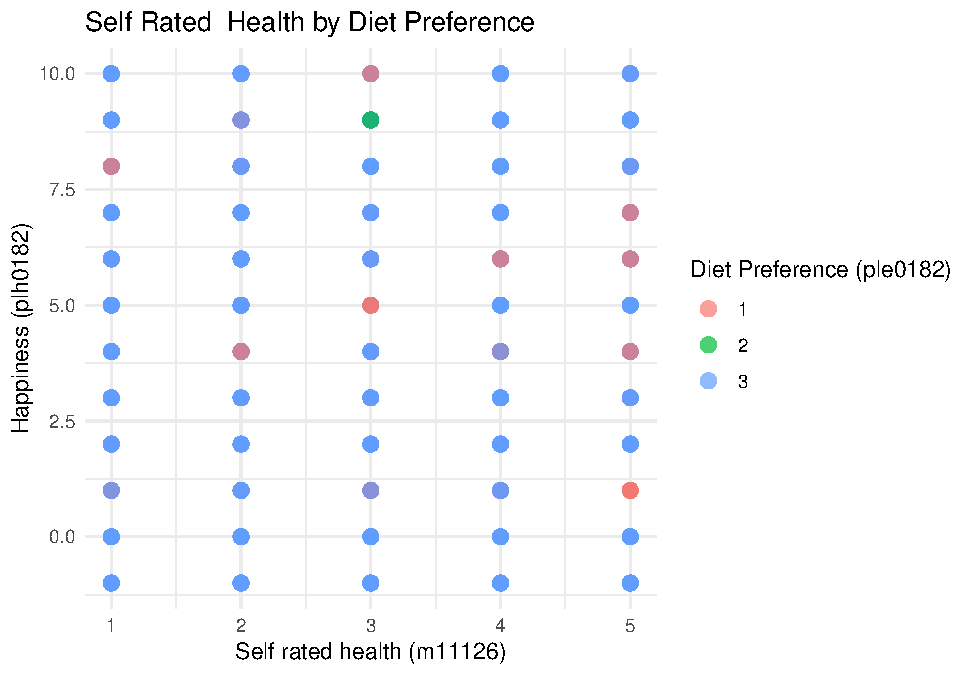
\includegraphics{Final-v2_files/figure-latex/self health~analysis-1.pdf}

From the graph, it is evident that non-vegetarians (Diet Preference 3,
blue) generally dominate across all levels of self-rated health, with a
significant presence at both lower and higher happiness scores. This
suggests that non-vegetarians, regardless of how they rate their own
health, experience a wide range of happiness levels, indicating that
factors other than self-perceived health might be influencing their
overall happiness.

Vegetarians (Diet Preference 1, red) and vegans (Diet Preference 2,
green) are more sparsely distributed across the health ratings.
Vegetarians, in particular, seem to cluster more in the mid to higher
self-rated health categories (3 to 5), often reporting higher happiness
scores as their self-rated health improves. This suggests that
vegetarians who consider themselves healthier are more likely to report
greater happiness.

Interestingly, vegans, while fewer in number, occasionally report very
high happiness scores even at mid-levels of self-rated health. This
indicates that vegans' happiness might be less directly tied to their
self-rated health compared to vegetarians and non-vegetarians,
potentially reflecting other contributing factors to their well-being.

\textbf{Outliers:} There are some low happiness scores among individuals
with high self-rated health, particularly among non-vegetarians, which
could be seen as outliers since better health typically correlates with
higher happiness.

\subsection{Individual Analysis}\label{individual-analysis}

The following graphs are plotted and analysed just with the variable and
dietary preference.

\subsubsection{Education and
vegetarinism}\label{education-and-vegetarinism}

This analysis aims to explore the relationship between an individual's
education level and their reported happiness, under the assumption that
higher education levels might correlate with greater happiness. The
rationale behind this assumption is that higher education often provides
individuals with better opportunities, higher income potential, and
greater personal fulfillment, all of which could contribute to increased
life satisfaction and happiness.

\begin{Shaded}
\begin{Highlighting}[]
\CommentTok{\# Load the data}
\NormalTok{pl\_education }\OtherTok{\textless{}{-}} \FunctionTok{read\_dta}\NormalTok{(}\StringTok{"pl.dta"}\NormalTok{, }\AttributeTok{col\_select =} \FunctionTok{c}\NormalTok{(}\StringTok{"pid"}\NormalTok{, }\StringTok{"syear"}\NormalTok{, }\StringTok{"ple0182"}\NormalTok{, }\StringTok{"plh0182"}\NormalTok{))}
\NormalTok{pequiv\_education }\OtherTok{\textless{}{-}} \FunctionTok{read\_dta}\NormalTok{(}\StringTok{"pequiv.dta"}\NormalTok{, }\AttributeTok{col\_select =} \FunctionTok{c}\NormalTok{(}\StringTok{"pid"}\NormalTok{, }\StringTok{"d11108"}\NormalTok{))}

\CommentTok{\# Exclusion values}
\NormalTok{exclusion\_values }\OtherTok{\textless{}{-}} \FunctionTok{c}\NormalTok{(}\SpecialCharTok{{-}}\DecValTok{1}\NormalTok{, }\SpecialCharTok{{-}}\DecValTok{2}\NormalTok{, }\SpecialCharTok{{-}}\DecValTok{3}\NormalTok{, }\SpecialCharTok{{-}}\DecValTok{4}\NormalTok{, }\SpecialCharTok{{-}}\DecValTok{5}\NormalTok{, }\SpecialCharTok{{-}}\DecValTok{6}\NormalTok{, }\SpecialCharTok{{-}}\DecValTok{7}\NormalTok{, }\SpecialCharTok{{-}}\DecValTok{8}\NormalTok{)}

\NormalTok{pl\_education}\OtherTok{\textless{}{-}}\NormalTok{ pl\_education[}\SpecialCharTok{!}\NormalTok{pl\_education}\SpecialCharTok{$}\NormalTok{ple0182 }\SpecialCharTok{\%in\%}\NormalTok{ exclusion\_values, ]}

\CommentTok{\# Remove rows with exclusion values in the m11126 column from pgen\_income}
\NormalTok{pequiv\_education }\OtherTok{\textless{}{-}}\NormalTok{ pequiv\_education[}\SpecialCharTok{!}\NormalTok{pequiv\_education}\SpecialCharTok{$}\NormalTok{d11108 }\SpecialCharTok{\%in\%}\NormalTok{ exclusion\_values, ]}

\CommentTok{\# Merge the education}
\NormalTok{merged\_education }\OtherTok{\textless{}{-}} \FunctionTok{merge}\NormalTok{(pl\_health, pequiv\_education, }\AttributeTok{by =} \StringTok{"pid"}\NormalTok{, }\AttributeTok{all.x =} \ConstantTok{TRUE}\NormalTok{)}



\NormalTok{merged\_education}\SpecialCharTok{$}\NormalTok{ple0182 }\OtherTok{\textless{}{-}} \FunctionTok{factor}\NormalTok{(merged\_education}\SpecialCharTok{$}\NormalTok{ple0182, }
                                \AttributeTok{levels =} \FunctionTok{c}\NormalTok{(}\DecValTok{1}\NormalTok{, }\DecValTok{2}\NormalTok{, }\DecValTok{3}\NormalTok{),}
                                \AttributeTok{labels =} \FunctionTok{c}\NormalTok{(}\StringTok{"Vegetarian"}\NormalTok{, }\StringTok{"Vegan"}\NormalTok{, }\StringTok{"Meat Eater"}\NormalTok{))}

\CommentTok{\# Violin plot}
\FunctionTok{ggplot}\NormalTok{(merged\_education, }\FunctionTok{aes}\NormalTok{(}\AttributeTok{x =}\NormalTok{ ple0182, }\AttributeTok{y =}\NormalTok{ d11108, }\AttributeTok{fill =}\NormalTok{ ple0182)) }\SpecialCharTok{+}
  \FunctionTok{geom\_violin}\NormalTok{(}\AttributeTok{trim =} \ConstantTok{FALSE}\NormalTok{) }\SpecialCharTok{+}
  \FunctionTok{labs}\NormalTok{(}\AttributeTok{title =} \StringTok{" Diet Preference by Education Level "}\NormalTok{,}
       \AttributeTok{x =} \StringTok{"Diet Preference"}\NormalTok{,}
       \AttributeTok{y =} \StringTok{"Education Level (d11108)"}\NormalTok{,}
       \AttributeTok{fill =} \StringTok{"Diet Preference"}\NormalTok{) }\SpecialCharTok{+}
  \FunctionTok{theme\_minimal}\NormalTok{()}
\end{Highlighting}
\end{Shaded}

\includegraphics{Final-v2_files/figure-latex/Education~analysis-1.pdf}

This graph illustrates the distribution of education levels across
different diet preferences, specifically for vegetarians, vegans, and
meat eaters. The x-axis represents the three diet categories, while the
y-axis shows the education levels. Each violin plot displays the spread
and density of individuals within each diet group according to their
education level.

From the graph, it is evident that vegans (green) generally have higher
education levels compared to vegetarians (red) and meat eaters (blue).
Vegans show a strong concentration at the upper end of the education
spectrum, particularly around level 3, indicating that a significant
portion of vegans have attained higher education. Vegetarians also tend
to have higher education levels, though their distribution shows a more
balanced presence between levels 2 and 3, with fewer individuals at the
lowest education level.

Meat eaters, on the other hand, exhibit a more even distribution across
the education spectrum, with a noticeable concentration around level 2.
This suggests that meat eaters come from a broader range of educational
backgrounds, with representation across both lower and higher education
levels.

The shape and spread of these violin plots suggest that higher education
levels are more closely associated with vegetarian and vegan diets,
while meat eaters tend to have a more diverse range of educational
backgrounds. This distribution implies that educational attainment may
influence dietary choices, with individuals who have higher education
being more likely to adopt vegetarian or vegan diets.

\textbf{Outliers:} The plot suggests a concentration at the extremes
(e.g., vegetarians at the highest education level), but these are not
necessarily outliers---they represent the distribution within each
group. 7. Diet Preferen

\subsubsection{Relegion and
Vegetarinism}\label{relegion-and-vegetarinism}

Often our dietary choices are made up by relegion/relegious backgraound
we were raised in.Some relegion prohibits eating certain/all meats or
plants(Jainism-root based vegetables). Analyzing the relationship
between religion and vegetarianism highlights the ethical dimensions of
dietary choices and how they are influenced by religious teachings.

\begin{Shaded}
\begin{Highlighting}[]
\CommentTok{\# Read the data}
\NormalTok{pl\_relegion }\OtherTok{\textless{}{-}} \FunctionTok{read\_dta}\NormalTok{(}\StringTok{"pl.dta"}\NormalTok{, }\AttributeTok{col\_select =} \FunctionTok{c}\NormalTok{(}\StringTok{"pid"}\NormalTok{, }\StringTok{"syear"}\NormalTok{, }\StringTok{"ple0182"}\NormalTok{, }\StringTok{"plh0182"}\NormalTok{,}\StringTok{"plh0258\_h"}\NormalTok{))}

\CommentTok{\# Exclusion values}
\NormalTok{exclusion\_values }\OtherTok{\textless{}{-}} \FunctionTok{c}\NormalTok{(}\SpecialCharTok{{-}}\DecValTok{1}\NormalTok{, }\SpecialCharTok{{-}}\DecValTok{2}\NormalTok{, }\SpecialCharTok{{-}}\DecValTok{3}\NormalTok{, }\SpecialCharTok{{-}}\DecValTok{4}\NormalTok{, }\SpecialCharTok{{-}}\DecValTok{5}\NormalTok{, }\SpecialCharTok{{-}}\DecValTok{6}\NormalTok{, }\SpecialCharTok{{-}}\DecValTok{7}\NormalTok{, }\SpecialCharTok{{-}}\DecValTok{8}\NormalTok{)}

\CommentTok{\# Remove rows with exclusion values in plb0592 column}
\NormalTok{pl\_relegion }\OtherTok{\textless{}{-}}\NormalTok{ pl\_relegion[}\SpecialCharTok{!}\NormalTok{pl\_relegion}\SpecialCharTok{$}\NormalTok{ple0182 }\SpecialCharTok{\%in\%}\NormalTok{ exclusion\_values, ]}

\CommentTok{\# Remove rows with exclusion values in plb0585 column}
\NormalTok{pl\_relegion }\OtherTok{\textless{}{-}}\NormalTok{ pl\_relegion[}\SpecialCharTok{!}\NormalTok{pl\_relegion}\SpecialCharTok{$}\NormalTok{plh0258\_h }\SpecialCharTok{\%in\%}\NormalTok{ exclusion\_values, ]}

\CommentTok{\# Map religion and diet preference codes to their respective labels}
\NormalTok{pl\_relegion}\SpecialCharTok{$}\NormalTok{ple0182 }\OtherTok{\textless{}{-}} \FunctionTok{factor}\NormalTok{(pl\_relegion}\SpecialCharTok{$}\NormalTok{ple0182, }
                              \AttributeTok{levels =} \FunctionTok{c}\NormalTok{(}\DecValTok{1}\NormalTok{, }\DecValTok{2}\NormalTok{, }\DecValTok{3}\NormalTok{),}
                              \AttributeTok{labels =} \FunctionTok{c}\NormalTok{(}\StringTok{"Vegetarian"}\NormalTok{, }\StringTok{"Vegan"}\NormalTok{, }\StringTok{"Meat Eater"}\NormalTok{))}

\NormalTok{pl\_relegion}\SpecialCharTok{$}\NormalTok{plh0258\_h }\OtherTok{\textless{}{-}} \FunctionTok{factor}\NormalTok{(pl\_relegion}\SpecialCharTok{$}\NormalTok{plh0258\_h, }
                                \AttributeTok{levels =} \DecValTok{1}\SpecialCharTok{:}\DecValTok{11}\NormalTok{,}
                                \AttributeTok{labels =} \FunctionTok{c}\NormalTok{(}\StringTok{"Katholisch"}\NormalTok{, }
                                           \StringTok{"Evangelisch"}\NormalTok{, }
                                           \StringTok{"Andere christlische Religionsgemeinschaft"}\NormalTok{,}
                                           \StringTok{"Islamische Religionsgemeinschaft"}\NormalTok{, }
                                           \StringTok{"Andere Religionsgemeinschaft"}\NormalTok{,}
                                           \StringTok{"Konfessionslos"}\NormalTok{, }
                                           \StringTok{"Christlich orthodox"}\NormalTok{, }
                                           \StringTok{"Schiitische Rel.gemeinschaft"}\NormalTok{,}
                                           \StringTok{"Sunnitische Rel.gemeinschaft"}\NormalTok{, }
                                           \StringTok{"Alevitische Rel.gemeinschaft"}\NormalTok{,}
                                           \StringTok{"Mehrfachnennung"}\NormalTok{))}

\CommentTok{\# Create a bar plot}
\FunctionTok{ggplot}\NormalTok{(pl\_relegion, }\FunctionTok{aes}\NormalTok{(}\AttributeTok{x =}\NormalTok{ plh0258\_h, }\AttributeTok{fill =}\NormalTok{ ple0182)) }\SpecialCharTok{+}
  \FunctionTok{geom\_bar}\NormalTok{(}\AttributeTok{position =} \StringTok{"dodge"}\NormalTok{) }\SpecialCharTok{+}
  \FunctionTok{labs}\NormalTok{(}\AttributeTok{title =} \StringTok{"Diet Preference by Religion"}\NormalTok{,}
       \AttributeTok{x =} \StringTok{"Religion"}\NormalTok{,}
       \AttributeTok{y =} \StringTok{"Count"}\NormalTok{,}
       
       
       \AttributeTok{fill =} \StringTok{"Diet Preference"}\NormalTok{) }\SpecialCharTok{+}
  \FunctionTok{theme\_minimal}\NormalTok{() }\SpecialCharTok{+}
  \FunctionTok{theme}\NormalTok{(}\AttributeTok{axis.text.x =} \FunctionTok{element\_text}\NormalTok{(}\AttributeTok{angle =} \DecValTok{45}\NormalTok{, }\AttributeTok{hjust =} \DecValTok{1}\NormalTok{))}
\end{Highlighting}
\end{Shaded}

\includegraphics{Final-v2_files/figure-latex/Relegion~analysis-1.pdf}

From the graph, it is evident that meat eaters (represented by the
turquoise bars) significantly outnumber vegans (represented by the red
bars) across all religious groups. The highest concentration of meat
eaters is found within the ``Sunnitische Religionsgemeinschaft'' (Sunni
Religious Community), followed by ``Katholisch'' (Catholic) and
``Konfessionslos'' (Non-religious/No affiliation). These groups show a
strong preference for a meat-based diet, with very few individuals
identifying as vegan.

Vegans are sparsely represented across the religions, with a small
presence in the ``Konfessionslos'' category and a minimal appearance in
``Andere Religionsgemeinschaft'' (Other Religious Communities). This
suggests that veganism is relatively uncommon within most religious
groups represented in this dataset.

Surprisingly,There are no complete vegetarians in this dataset.

Overall, the graph indicates that religious affiliation may influence
dietary preferences, with a dominant trend toward meat consumption
across all religious groups. The limited representation of vegans
suggests that either veganism is less prevalent among individuals within
these religious affiliations, or that other factors, such as cultural or
societal norms within these groups, may also play a role in shaping diet
preferences.

\textbf{Outliers:} The low representation of vegans and \textbf{\emph{0
representation of vegetarians}} across most religions could be
considered an outlier, but this is more a reflection of actual
distribution rather than an anomalous data point.

\subsubsection{Survey Year and
Vegetarinism}\label{survey-year-and-vegetarinism}

This plot tries to find out if the mean happiness is increasing,while
\textbf{\emph{ceteris paribus(Other things remaining the
same).}}Analyzing how mean happiness changes over different survey years
can help identify broader societal trends in well-being. If mean
happiness is increasing or decreasing over time, it could reflect
changes in societal conditions, economic factors, political stability,
or cultural shifts that impact overall life satisfaction.

When analyzing mean happiness while holding other factors constant
\textbf{\emph{(ceteris paribus),}} you can isolate the effect of time
itself on happiness. This helps determine whether happiness is
inherently trending upwards or downwards over time, independent of other
variables.

\begin{Shaded}
\begin{Highlighting}[]
\CommentTok{\# Assuming merged\_data already includes \textquotesingle{}syear\textquotesingle{} and \textquotesingle{}plh0182\textquotesingle{} (happiness scores)}
\CommentTok{\# Group by survey year and calculate mean happiness}
\NormalTok{yearly\_happiness }\OtherTok{\textless{}{-}}\NormalTok{ merged\_data }\SpecialCharTok{\%\textgreater{}\%}
  \FunctionTok{group\_by}\NormalTok{(syear) }\SpecialCharTok{\%\textgreater{}\%}
  \FunctionTok{summarise}\NormalTok{(}\AttributeTok{mean\_happiness =} \FunctionTok{mean}\NormalTok{(plh0182, }\AttributeTok{na.rm =} \ConstantTok{TRUE}\NormalTok{),  }\CommentTok{\# Remove NA values for accurate calculation}
            \AttributeTok{.groups =} \StringTok{\textquotesingle{}drop\textquotesingle{}}\NormalTok{)  }\CommentTok{\# This option drops the grouping after summarization}


\FunctionTok{ggplot}\NormalTok{(yearly\_happiness, }\FunctionTok{aes}\NormalTok{(}\AttributeTok{x =}\NormalTok{ syear, }\AttributeTok{y =}\NormalTok{ mean\_happiness)) }\SpecialCharTok{+}
  \FunctionTok{geom\_line}\NormalTok{(}\AttributeTok{group =} \DecValTok{1}\NormalTok{, }\AttributeTok{color =} \StringTok{"blue"}\NormalTok{) }\SpecialCharTok{+}  \CommentTok{\# Connect points with a line}
  \FunctionTok{geom\_point}\NormalTok{(}\AttributeTok{color =} \StringTok{"red"}\NormalTok{, }\AttributeTok{size =} \DecValTok{3}\NormalTok{) }\SpecialCharTok{+}  \CommentTok{\# Add points to each year\textquotesingle{}s mean happiness}
  \FunctionTok{labs}\NormalTok{(}\AttributeTok{title =} \StringTok{"Mean Happiness Score by Survey Year"}\NormalTok{,}
       \AttributeTok{x =} \StringTok{"Survey Year"}\NormalTok{,}
       \AttributeTok{y =} \StringTok{"Mean Happiness Score"}\NormalTok{) }\SpecialCharTok{+}
  \FunctionTok{theme\_minimal}\NormalTok{() }\SpecialCharTok{+}
  \FunctionTok{theme}\NormalTok{(}\AttributeTok{plot.title =} \FunctionTok{element\_text}\NormalTok{(}\AttributeTok{hjust =} \FloatTok{0.5}\NormalTok{),}
        \AttributeTok{axis.title.x =} \FunctionTok{element\_text}\NormalTok{(}\AttributeTok{vjust =} \SpecialCharTok{{-}}\FloatTok{0.2}\NormalTok{),}
        \AttributeTok{axis.title.y =} \FunctionTok{element\_text}\NormalTok{(}\AttributeTok{vjust =} \DecValTok{2}\NormalTok{))}
\end{Highlighting}
\end{Shaded}

\includegraphics{Final-v2_files/figure-latex/Survey yearanalysis-1.pdf}

From the graph, it is evident that mean happiness scores have been
steadily increasing over the period from 2016 to 2020. Starting from a
mean happiness score of around 7.30 in 2016, there is a noticeable
upward trend, reaching approximately 7.50 by 2020. This consistent rise
suggests an overall improvement in happiness levels among the surveyed
population over these years.

The linear nature of the trend line indicates a fairly uniform increase
in happiness, without significant fluctuations or deviations. This could
imply that whatever factors are contributing to increased happiness,
they have been steadily improving or consistently impacting the
population in a positive manner during this period.

\textbf{Outliers:}There are no visible outliers, as the trend is linear
and consistent without any abrupt changes or deviations.

\subsubsection{Overall Satisfaction and
Vegatrinism}\label{overall-satisfaction-and-vegatrinism}

Inorder to see the validity of finidngs in Current life satisfaction,I
took Overall life satisfaction for a sepertae analysis.If the
relationship between vegetarianism and happiness remains consistent when
using both ``Current Life Satisfaction'' and ``Overall Life
Satisfaction,'' this suggests that the impact of vegetarianism on
happiness is stable over both short-term (current) and long-term
(overall) perspectives. This consistency would strengthen the validity
of findings, indicating that vegetarianism has a sustained impact on an
individual's overall well-being.

\begin{Shaded}
\begin{Highlighting}[]
\CommentTok{\# Load the data}
\NormalTok{pl\_overall }\OtherTok{\textless{}{-}} \FunctionTok{read\_dta}\NormalTok{(}\StringTok{"pl.dta"}\NormalTok{, }\AttributeTok{col\_select =} \FunctionTok{c}\NormalTok{(}\StringTok{"pid"}\NormalTok{, }\StringTok{"syear"}\NormalTok{, }\StringTok{"ple0182"}\NormalTok{, }\StringTok{"plh0182"}\NormalTok{))}
\NormalTok{pequiv\_overall }\OtherTok{\textless{}{-}} \FunctionTok{read\_dta}\NormalTok{(}\StringTok{"pequiv.dta"}\NormalTok{, }\AttributeTok{col\_select =} \FunctionTok{c}\NormalTok{(}\StringTok{"pid"}\NormalTok{, }\StringTok{"p11101"}\NormalTok{))}

\CommentTok{\# Exclusion values}
\NormalTok{exclusion\_values }\OtherTok{\textless{}{-}} \FunctionTok{c}\NormalTok{(}\SpecialCharTok{{-}}\DecValTok{1}\NormalTok{, }\SpecialCharTok{{-}}\DecValTok{2}\NormalTok{, }\SpecialCharTok{{-}}\DecValTok{3}\NormalTok{, }\SpecialCharTok{{-}}\DecValTok{4}\NormalTok{, }\SpecialCharTok{{-}}\DecValTok{5}\NormalTok{, }\SpecialCharTok{{-}}\DecValTok{6}\NormalTok{, }\SpecialCharTok{{-}}\DecValTok{7}\NormalTok{, }\SpecialCharTok{{-}}\DecValTok{8}\NormalTok{)}

\NormalTok{pl\_overall}\OtherTok{\textless{}{-}}\NormalTok{ pl\_overall[}\SpecialCharTok{!}\NormalTok{pl\_overall}\SpecialCharTok{$}\NormalTok{ple0182 }\SpecialCharTok{\%in\%}\NormalTok{ exclusion\_values, ]}

\CommentTok{\# Remove rows with exclusion values in the m11126 column from pgen\_income}
\NormalTok{pequiv\_overall }\OtherTok{\textless{}{-}}\NormalTok{ pequiv\_overall[}\SpecialCharTok{!}\NormalTok{pequiv\_overall}\SpecialCharTok{$}\NormalTok{p11101 }\SpecialCharTok{\%in\%}\NormalTok{ exclusion\_values, ]}

\CommentTok{\# Merge the education}
\NormalTok{merged\_overall }\OtherTok{\textless{}{-}} \FunctionTok{merge}\NormalTok{(pl\_overall, pequiv\_overall, }\AttributeTok{by =} \StringTok{"pid"}\NormalTok{, }\AttributeTok{all.x =} \ConstantTok{TRUE}\NormalTok{)}



\NormalTok{merged\_overall}\SpecialCharTok{$}\NormalTok{ple0182 }\OtherTok{\textless{}{-}} \FunctionTok{factor}\NormalTok{(merged\_overall}\SpecialCharTok{$}\NormalTok{ple0182, }
                                \AttributeTok{levels =} \FunctionTok{c}\NormalTok{(}\DecValTok{1}\NormalTok{, }\DecValTok{2}\NormalTok{, }\DecValTok{3}\NormalTok{),}
                                \AttributeTok{labels =} \FunctionTok{c}\NormalTok{(}\StringTok{"Vegetarian"}\NormalTok{, }\StringTok{"Vegan"}\NormalTok{, }\StringTok{"Meat Eater"}\NormalTok{))}



\CommentTok{\# Calculate the mean p11101 for each diet preference}
\NormalTok{mean\_values }\OtherTok{\textless{}{-}}\NormalTok{ merged\_overall }\SpecialCharTok{\%\textgreater{}\%}
  \FunctionTok{group\_by}\NormalTok{(ple0182) }\SpecialCharTok{\%\textgreater{}\%}
  \FunctionTok{summarise}\NormalTok{(}\AttributeTok{mean\_p11101 =} \FunctionTok{mean}\NormalTok{(p11101, }\AttributeTok{na.rm =} \ConstantTok{TRUE}\NormalTok{))}

\CommentTok{\# Display the table}
\NormalTok{mean\_values}
\end{Highlighting}
\end{Shaded}

\begin{verbatim}
## # A tibble: 3 x 2
##   ple0182    mean_p11101
##   <fct>            <dbl>
## 1 Vegetarian        7.47
## 2 Vegan             7.49
## 3 Meat Eater        7.29
\end{verbatim}

\begin{Shaded}
\begin{Highlighting}[]
\CommentTok{\# Calculate the mean p11101 for each diet preference}
\NormalTok{mean\_p11101 }\OtherTok{\textless{}{-}}\NormalTok{ merged\_overall }\SpecialCharTok{\%\textgreater{}\%}
  \FunctionTok{group\_by}\NormalTok{(ple0182) }\SpecialCharTok{\%\textgreater{}\%}
  \FunctionTok{summarise}\NormalTok{(}\AttributeTok{mean\_p11101 =} \FunctionTok{mean}\NormalTok{(p11101, }\AttributeTok{na.rm =} \ConstantTok{TRUE}\NormalTok{))}

\CommentTok{\# Create a bar plot}
\FunctionTok{ggplot}\NormalTok{(mean\_p11101, }\FunctionTok{aes}\NormalTok{(}\AttributeTok{x =}\NormalTok{ ple0182, }\AttributeTok{y =}\NormalTok{ mean\_p11101, }\AttributeTok{fill =}\NormalTok{ ple0182)) }\SpecialCharTok{+}
  \FunctionTok{geom\_bar}\NormalTok{(}\AttributeTok{stat =} \StringTok{"identity"}\NormalTok{) }\SpecialCharTok{+}
  \FunctionTok{labs}\NormalTok{(}\AttributeTok{title =} \StringTok{"Overall Life satisfaction by Diet Preference"}\NormalTok{,}
       \AttributeTok{x =} \StringTok{"Diet Preference"}\NormalTok{,}
       \AttributeTok{y =} \StringTok{"Mean p11101"}\NormalTok{,}
       \AttributeTok{fill =} \StringTok{"Diet Preference"}\NormalTok{) }\SpecialCharTok{+}
  \FunctionTok{theme\_minimal}\NormalTok{()}
\end{Highlighting}
\end{Shaded}

\includegraphics{Final-v2_files/figure-latex/Overall satisfaction ~analysis-1.pdf}

This bar chart illustrates the mean overall life satisfaction (labeled
as p11101) across different diet preferences: Vegetarian (red), Vegan
(green), and Meat Eater (blue). The x-axis categorizes the diet types,
while the y-axis shows the mean overall life satisfaction score for each
group.

From the graph, it is evident that vegetarians and vegans report
slightly higher mean overall life satisfaction compared to meat eaters.
The mean life satisfaction scores for vegetarians and vegans are nearly
identical, both slightly higher than the score for meat eaters.

This suggests that, on average, individuals who follow a vegetarian or
vegan diet tend to report higher overall life satisfaction than those
who consume meat. The differences, however, are not drastic, indicating
that while diet preference might have some influence on life
satisfaction, it may not be the sole determining factor. Other variables
such as personal values, health, and lifestyle could also play
significant roles in shaping an individual's overall sense of
well-being.

\textbf{Outliers:} There are no visible outliers, as the scores are
quite uniform across the diet groups.

\subsection{Vegetarinism and Current-life
satisfaction(Happiness)}\label{vegetarinism-and-current-life-satisfactionhappiness}

\begin{Shaded}
\begin{Highlighting}[]
\CommentTok{\# Assuming pl is loaded}
\CommentTok{\# Transform pl to include DietType}
\NormalTok{pl }\OtherTok{\textless{}{-}}\NormalTok{ pl }\SpecialCharTok{\%\textgreater{}\%}
  \FunctionTok{mutate}\NormalTok{(}\AttributeTok{DietType =} \FunctionTok{case\_when}\NormalTok{(}
\NormalTok{    ple0182 }\SpecialCharTok{==} \DecValTok{1} \SpecialCharTok{\textasciitilde{}} \StringTok{"Vegetarian"}\NormalTok{,}
\NormalTok{    ple0182 }\SpecialCharTok{==} \DecValTok{2} \SpecialCharTok{\textasciitilde{}} \StringTok{"Vegan"}\NormalTok{,}
\NormalTok{    ple0182 }\SpecialCharTok{==} \DecValTok{3} \SpecialCharTok{\textasciitilde{}} \StringTok{"Non{-}vegetarian"}
\NormalTok{  ))}

\CommentTok{\# Filter for relevant diet types}
\NormalTok{pl\_filtered }\OtherTok{\textless{}{-}}\NormalTok{ pl[pl}\SpecialCharTok{$}\NormalTok{ple0182 }\SpecialCharTok{\%in\%} \FunctionTok{c}\NormalTok{(}\DecValTok{1}\NormalTok{, }\DecValTok{2}\NormalTok{, }\DecValTok{3}\NormalTok{), ]}

\CommentTok{\# Plotting with points and a smooth trend line}
\FunctionTok{ggplot}\NormalTok{(pl\_filtered, }\FunctionTok{aes}\NormalTok{(}\AttributeTok{x =}\NormalTok{ DietType, }\AttributeTok{y =}\NormalTok{ pl\_filtered}\SpecialCharTok{$}\NormalTok{plh0182, }\AttributeTok{color =}\NormalTok{ DietType)) }\SpecialCharTok{+}
  \FunctionTok{geom\_point}\NormalTok{(}\AttributeTok{alpha =} \FloatTok{0.6}\NormalTok{, }\AttributeTok{position =} \FunctionTok{position\_jitter}\NormalTok{(}\AttributeTok{width =} \FloatTok{0.2}\NormalTok{), }\AttributeTok{size =} \DecValTok{2}\NormalTok{) }\SpecialCharTok{+}
  \FunctionTok{geom\_smooth}\NormalTok{(}\AttributeTok{method =} \StringTok{"loess"}\NormalTok{, }\AttributeTok{se =} \ConstantTok{FALSE}\NormalTok{, }\AttributeTok{color =} \StringTok{"black"}\NormalTok{) }\SpecialCharTok{+}
  \FunctionTok{scale\_color\_manual}\NormalTok{(}\AttributeTok{values =} \FunctionTok{c}\NormalTok{(}\StringTok{"Vegetarian"} \OtherTok{=} \StringTok{"green"}\NormalTok{, }\StringTok{"Vegan"} \OtherTok{=} \StringTok{"purple"}\NormalTok{, }\StringTok{"Non{-}vegetarian"} \OtherTok{=} \StringTok{"gray"}\NormalTok{)) }\SpecialCharTok{+}
  \FunctionTok{labs}\NormalTok{(}\AttributeTok{x =} \StringTok{"Diet Type"}\NormalTok{, }\AttributeTok{y =} \StringTok{"Happiness Score"}\NormalTok{,}
       \AttributeTok{title =} \StringTok{"Happiness Scores by Diet Type"}\NormalTok{,}
       \AttributeTok{subtitle =} \StringTok{"Point distribution and trend lines across diet types"}\NormalTok{,}
       \AttributeTok{caption =} \StringTok{"Data source: Survey Data"}\NormalTok{) }\SpecialCharTok{+}
  \FunctionTok{theme\_minimal}\NormalTok{() }\SpecialCharTok{+}
  \FunctionTok{theme}\NormalTok{(}\AttributeTok{plot.title =} \FunctionTok{element\_text}\NormalTok{(}\AttributeTok{hjust =} \FloatTok{0.5}\NormalTok{),}
        \AttributeTok{plot.subtitle =} \FunctionTok{element\_text}\NormalTok{(}\AttributeTok{hjust =} \FloatTok{0.5}\NormalTok{),}
        \AttributeTok{plot.caption =} \FunctionTok{element\_text}\NormalTok{(}\AttributeTok{hjust =} \DecValTok{1}\NormalTok{),}
        \AttributeTok{legend.position =} \StringTok{"top"}\NormalTok{,}
        \AttributeTok{axis.text.x =} \FunctionTok{element\_text}\NormalTok{(}\AttributeTok{angle =} \DecValTok{45}\NormalTok{, }\AttributeTok{hjust =} \DecValTok{1}\NormalTok{))}
\end{Highlighting}
\end{Shaded}

\includegraphics{Final-v2_files/figure-latex/Veg~analysis-1.pdf}

This scatter plot shows the distribution of happiness scores across
different diet types: Non-vegetarian (gray), Vegan (purple), and
Vegetarian (green). The x-axis represents the diet types, while the
y-axis indicates the happiness scores, which range from 0 to 10.

From the graph, it is evident that happiness scores vary widely within
each diet group, but some patterns emerge:

Non-vegetarians (Gray): The happiness scores for non-vegetarians are
spread across the entire range from 0 to 10, with a dense cluster
between the mid to high range (around 5 to 10). This suggests that
non-vegetarians experience a broad spectrum of happiness levels, though
many report relatively high scores.

Vegans (Purple): Vegans also display a wide distribution of happiness
scores, but with a noticeable concentration towards the higher end of
the scale (around 7 to 10). This concentration indicates that a
significant proportion of vegans report higher levels of happiness.

Vegetarians (Green): Similar to vegans, vegetarians tend to report
higher happiness scores, with many scores clustering between 7 and 10.
However, there is also a wider spread towards lower happiness scores
compared to vegans, indicating more variability in how vegetarians
perceive their happiness.

Overall, the graph suggests that while happiness scores are widely
distributed within each diet group, vegans and vegetarians tend to
report higher happiness levels more consistently than non-vegetarians.
The clustering of higher scores among vegans and vegetarians might
suggest that these diet types are associated with greater overall
happiness, though individual experiences vary significantly within all
groups.

\textbf{Outliers:} Some very low happiness scores among non-vegetarians,
especially given the wide spread, could be considered outliers, as well
as some high happiness scores among individuals with low self-rated
health.

\begin{Shaded}
\begin{Highlighting}[]
\CommentTok{\# Group by DietType and calculate average happiness}
\NormalTok{average\_happiness }\OtherTok{\textless{}{-}}\NormalTok{ pl\_filtered }\SpecialCharTok{\%\textgreater{}\%}
  \FunctionTok{group\_by}\NormalTok{(DietType) }\SpecialCharTok{\%\textgreater{}\%}
  \FunctionTok{summarise}\NormalTok{(}\AttributeTok{AverageHappiness =} \FunctionTok{mean}\NormalTok{(plh0182, }\AttributeTok{na.rm =} \ConstantTok{TRUE}\NormalTok{), }\AttributeTok{.groups =} \StringTok{\textquotesingle{}drop\textquotesingle{}}\NormalTok{)}

\CommentTok{\# Print out the results}
\FunctionTok{print}\NormalTok{(average\_happiness)}
\end{Highlighting}
\end{Shaded}

\begin{verbatim}
## # A tibble: 3 x 2
##   DietType       AverageHappiness
##   <chr>                     <dbl>
## 1 Non-vegetarian             7.46
## 2 Vegan                      7.69
## 3 Vegetarian                 7.53
\end{verbatim}

\begin{Shaded}
\begin{Highlighting}[]
\CommentTok{\# Plotting the average happiness levels}
\FunctionTok{ggplot}\NormalTok{(average\_happiness, }\FunctionTok{aes}\NormalTok{(}\AttributeTok{x =}\NormalTok{ DietType, }\AttributeTok{y =}\NormalTok{ AverageHappiness, }\AttributeTok{fill =}\NormalTok{ DietType)) }\SpecialCharTok{+}
  \FunctionTok{geom\_col}\NormalTok{() }\SpecialCharTok{+}
  \FunctionTok{scale\_fill\_manual}\NormalTok{(}\AttributeTok{values =} \FunctionTok{c}\NormalTok{(}\StringTok{"Vegetarian"} \OtherTok{=} \StringTok{"green"}\NormalTok{, }\StringTok{"Vegan"} \OtherTok{=} \StringTok{"purple"}\NormalTok{, }\StringTok{"Non{-}vegetarian"} \OtherTok{=} \StringTok{"gray"}\NormalTok{)) }\SpecialCharTok{+}
  \FunctionTok{labs}\NormalTok{(}\AttributeTok{x =} \StringTok{"Diet Type"}\NormalTok{, }\AttributeTok{y =} \StringTok{"Average Happiness Score"}\NormalTok{,}
       \AttributeTok{title =} \StringTok{"Average Happiness Scores by Diet Type"}\NormalTok{,}
       \AttributeTok{subtitle =} \StringTok{"Aggregated across all surveyed years"}\NormalTok{,}
       \AttributeTok{caption =} \StringTok{"Data source: Survey Data"}\NormalTok{) }\SpecialCharTok{+}
  \FunctionTok{theme\_minimal}\NormalTok{() }\SpecialCharTok{+}
  \FunctionTok{theme}\NormalTok{(}\AttributeTok{plot.title =} \FunctionTok{element\_text}\NormalTok{(}\AttributeTok{hjust =} \FloatTok{0.5}\NormalTok{),}
        \AttributeTok{plot.subtitle =} \FunctionTok{element\_text}\NormalTok{(}\AttributeTok{hjust =} \FloatTok{0.5}\NormalTok{),}
        \AttributeTok{plot.caption =} \FunctionTok{element\_text}\NormalTok{(}\AttributeTok{hjust =} \DecValTok{1}\NormalTok{),}
        \AttributeTok{legend.position =} \StringTok{"bottom"}\NormalTok{,}
        \AttributeTok{axis.text.x =} \FunctionTok{element\_text}\NormalTok{(}\AttributeTok{angle =} \DecValTok{45}\NormalTok{, }\AttributeTok{hjust =} \DecValTok{1}\NormalTok{))}
\end{Highlighting}
\end{Shaded}

\includegraphics{Final-v2_files/figure-latex/Fin-1.pdf}

From the graph, it is evident that all three diet
types---Non-vegetarian, Vegan, and Vegetarian---have similar average
happiness scores, with only minimal differences between them.
Non-vegetarians have a slightly lower average happiness score compared
to both vegans and vegetarians, who report nearly identical scores.

This suggests that, in general, diet type does not have a substantial
impact on happiness levels. Whether an individual is a non-vegetarian,
vegan, or vegetarian, their average happiness is relatively consistent.
The similarity in scores implies that other factors beyond diet may be
more influential in determining overall happiness, and that individuals
following different dietary patterns experience comparable levels of
well-being.

\section{Overall Life satisfaction and Current Life
satisfaction-assessment}\label{overall-life-satisfaction-and-current-life-satisfaction-assessment}

1.Small Differences Across Diet Types:

The figures indicate only slight variations in happiness scores across
the different diet types. This suggests that while there may be a
positive association between vegetarianism/veganism and happiness, the
effect size might be relatively modest. It implies that other factors
beyond diet---such as social support, health, or lifestyle
choices---might play more significant roles in influencing overall
happiness.

2.Validity of Findings:

The consistency across both measures (current and overall life
satisfaction) enhances the validity of your findings. It suggests that
the observed relationship between diet and happiness is not an artifact
of the time frame but rather a genuine, enduring effect.

3.Conclusion: The consistent findings between ``Current Life
Satisfaction'' and ``Overall Life Satisfaction'' suggest that the
positive impact of vegetarianism and veganism on happiness is stable
over both short-term and long-term perspectives. The similarity in
happiness scores across these two measures reinforces the validity of
the relationship, indicating that these dietary choices contribute to
sustained well-being. While the effect size appears modest, the
consistency suggests that vegetarianism and veganism have a genuine,
enduring positive influence on overall life satisfaction.

\section{Regression and Co-relation.}\label{regression-and-co-relation.}

The regression plot below illustrates the relationship between
`vegetarinism' and `Happiness'. Each scatter point represents an
individual observation from our estimation sample.

\includegraphics{Final-v2_files/figure-latex/Regression-1.pdf}

\begin{verbatim}
## [1] "Correlation coefficient: 0.0108671700092815"
\end{verbatim}

\includegraphics{Final-v2_files/figure-latex/Correlation-1.pdf}

\textbf{A correlation coefficient of 0.011} suggests that there is a
negligible positive linear relationship between `vegetarianism' and
`current life satisfaction'. However, the strength of this relationship
is extremely weak, implying that being vegetarian is only very slightly
associated with differences in `current life satisfaction'. This minimal
correlation indicates that dietary preference alone does not
significantly influence life satisfaction, and other factors likely play
a more substantial role in determining overall happiness.

\section{Presence of
Outliers-Summary}\label{presence-of-outliers-summary}

Across the figures, there are a few potential outliers, particularly in
the scatter plots where individuals report either significantly lower or
higher happiness than expected based on their income or self-rated
health. However, in the bar charts and trend lines, the data appears to
be consistent with no significant outliers. The overall patterns suggest
that while vegetarianism and veganism might have a positive influence on
happiness, the effect size is modest, and other factors also play a
significant role.

\section{Limitations and Next Steps for In-Depth
Analysis}\label{limitations-and-next-steps-for-in-depth-analysis}

\subsection{Limitations}\label{limitations}

\textbf{1.Despite the broader scope of this analysis}, limitations
remain, particularly in the depth of exploration into how these factors
interact with each other. Future research should focus on a more
detailed examination of the complex interplay between dietary choices
and other life satisfaction determinants, potentially employing more
advanced statistical techniques to capture these nuances.

\textbf{2.Also,vegetarinism was taken into consideration in soep
analysis only from 2016},and the data set where people responded in
1,2,3(Vegetarian,Vegan,Meat eating) preferences were low comparitevely.

\textbf{3.Cross-Sectional Nature:}The analysis is based on
cross-sectional data, meaning it captures a snapshot in time rather than
tracking changes over time. This limits the ability to draw causal
inferences or understand how the relationships between variables might
evolve.

\textbf{4.Self-Reported Data:}Variables like happiness and self-rated
health are based on self-reported data, which can be subjective and
prone to bias. Participants may overestimate or underestimate their
happiness or health, leading to inaccuracies in the analysis. Simplistic
Categorization:

\textbf{5.The categorization of diet preferences} (e.g., vegetarian,
vegan, non-vegetarian) may oversimplify the complexity of individuals'
dietary habits. For example, the ``non-vegetarian'' category includes a
wide range of diets that might have different impacts on happiness and
health. Potential Confounding Variables:

\subsection{Next Steps for In-Depth
Analysis:}\label{next-steps-for-in-depth-analysis}

\textbf{1.Conduct Longitudinal Studies:}

Implement a longitudinal study design to track changes in happiness,
health, and dietary habits over time. This would provide insights into
how sustained dietary choices impact long-term well-being. Include More
Demographic and Psychosocial Variables:

\textbf{2.Perform Multivariate Regression Analysis:}

Use multivariate regression models to control for confounding variables
and better isolate the effect of diet on happiness. This would help
determine whether the observed associations hold when other factors are
accounted for.

\textbf{3.Examine Sub-Groups Within Diet Categories:}

Break down the broad diet categories into more specific sub-groups
(e.g., pescatarian, flexitarian, whole-food plant-based) to explore
potential differences in their impact on happiness and health.

\textbf{4.Qualitative Research:}

Conduct qualitative research, such as interviews or focus groups, to
explore participants' motivations for their dietary choices and how
these relate to their perceptions of happiness and well-being. This
could provide deeper insights into the psychological and social factors
at play.

\textbf{5.Investigate Causal Relationships:}

Consider using experimental designs or instrumental variable approaches
to establish causal relationships between diet and happiness, rather
than merely observing associations.

\textbf{6.Explore Cultural and Geographic Differences:}

Expand the study to different cultural and geographic contexts to
understand how cultural norms and regional dietary patterns influence
the relationship between diet and happiness.

\section{Conclusion}\label{conclusion}

In conclusion, the analysis of the relationship between `vegetarianism'
and `current life satisfaction' based on the SOEP dataset has provided
valuable insights. Through data visualization, regression analysis, and
correlation, I have identified an extremely weak positive correlation
between `vegetarianism' and `current life satisfaction'. This suggests
that, on average, individuals who follow a vegetarian diet may have a
slightly different life satisfaction level compared to non-vegetarians.
However, the correlation coefficient value of 0.011 indicates that this
relationship is negligible and likely influenced by other factors not
considered in this analysis.

In this project, I have also taken into consideration \textbf{8
additional variables}, including age, gender, income, education, health,
religion, and overall life satisfaction, among others. The inclusion of
these variables allowed for a more comprehensive analysis, revealing
that while dietary preference may have some association with happiness,
it is likely overshadowed by the influence of other socio-economic and
demographic factors.

\section*{References}\label{references}
\addcontentsline{toc}{section}{References}

\phantomsection\label{refs}
\begin{CSLReferences}{1}{0}
\bibitem[\citeproctext]{ref-aslanifar2014comparison}
Aslanifar, E., Fakhri, M. K., Mirzaian, B., \& Babaei Kafaki, H. (2014).
\emph{The comparison of personality traits and happiness of vegetarians
and non-vegetarians}.

\bibitem[\citeproctext]{ref-beezhold2010vegetarian}
Beezhold, B. L., Johnston, C. S., \& Daigle, D. R. (2010). Vegetarian
diets are associated with healthy mood states: A cross-sectional study
in seventh day adventist adults. \emph{Nutrition Journal}, \emph{9}(26).
\url{https://doi.org/10.1186/1475-2891-9-26}

\bibitem[\citeproctext]{ref-goebel2019board}
Goebel, J., Grabka, M. M., Liebig, S., Kroh, M., Richter, D., Schröder,
C., \& Schupp, J. (2019). Board of directors SOEP and division head
applied panel analysis in the german socio-economic panel study
department. \emph{Jahrb{ü}cher f{ü}r National{ö}konomie Und Statistik},
\emph{239}(2), 345--360. \url{https://doi.org/10.1515/jbnst-2018-0022}

\bibitem[\citeproctext]{ref-pfeiler2018examining}
Pfeiler, T. M., \& Egloff, B. (2018). Examining the {``veggie''}
personality: Results from a representative german sample.
\emph{Appetite}, \emph{120}, 246--255.
\url{https://doi.org/10.1016/j.appet.2017.09.0052}

\bibitem[\citeproctext]{ref-rehder2023plant}
Rehder, L. (2023). \emph{Plant-based food goes mainstream in germany}
(GM2023-0002). U.S. Department of Agriculture Foreign Agricultural
Service. \url{https://www.fas.usda.gov}

\end{CSLReferences}

\end{document}
